\chapter{Related Work}
\label{chap:rel_work}

The realm of Linked Data, particularly in the context of digital art collections, has witnessed significant advancements. This chapter seeks to elucidate the foundational concepts and their real-world applications.

Section~\ref{sec:linked_data} provides an introduction to Linked Data, emphasizing its core principles, data modeling, and various RDF syntaxes. The section underscores the importance of unique URIs, dereferencing, and data interlinking.

In Section~\ref{sec:ltqp}, the spotlight is on Link-Traversal-based Query Processing (LTQP). Through an example, the intricacies of querying across different documents are unraveled, highlighting the challenges and the specific reachability criteria for link traversal.

Section~\ref{sec:comunica} delves into Comunica, a SPARQL query engine. The discussion revolves around its modularity, the foundational building blocks, and the potential to craft custom engine configurations tailored for distinct link traversal requirements.

Section~\ref{sec:coghent} presents the Collections of Ghent (CoGhent) initiative, a collaborative venture between cultural institutions in Ghent. The adoption of Linked Data Event Streams (LDES) for publishing digital collections is explored, alongside the CoGhent Query Builder application that aids in query formulation.

Concluding the chapter, Section~\ref{sec:iiif} introduces the International Image Interoperability Framework (IIIF). Namely, the role of IIIF Manifests and IIIF Viewers in the visualization of cultural data is discussed.

These sections provide the foundation for the subsequent chapters, which delve into various stages of a systematic process for discovering digital art collections. Each chapter builds upon the insights and methodologies presented in this chapter, ensuring a cohesive exploration throughout.

\section{Linked Data}
\label{sec:linked_data}

This section presents a comprehensive exploration of Linked Data, encompassing its fundamental principles, data modeling, syntax, query interfaces, and the associated challenges and advantages. In Section~\ref{subsec:introduction_principles}, the concept of Linked Data and its principles are introduced, highlighting the significance of unique URIs, dereferencing, and data interlinking. Section~\ref{subsec:rdf} focuses on the Resource Description Framework (RDF) as the cornerstone for representing relationships and knowledge connections within Linked Data. Section~\ref{subsec:rdf_syntax} provides an overview of RDF syntax, including popular formats such as XML, Turtle, N-Triples, and JSON-LD, which facilitate the flexible expression and exchange of RDF data. Lastly, Section~\ref{subsec:sparql} briefly introduces SPARQL, the query language for RDF data This comprehensive examination serves as a solid foundation for the subsequent discussions on Linked Traversal-based Query Processing.

\subsection{Introduction and Principles}
\label{subsec:introduction_principles}

To better understand the origins of the idea behind Linked Data, it is important to examine the origins of the World Wide Web. For example, its first, but still rather primitive, underlying technology was introduced in 1989 at CERN. Tim Berners-Lee was the man responsible for its development. By using HyperText Markup Language (HTML), it enabled scientists, and later the rest of the world, to publish documents that could contain links to other documents. This helped create a mesh of documents and information. However, since these documents in fact contained nothing more than raw data dumps and links between documents represented simply an indication of how to reach the document, these documents and their relationships lacked semantics. Figure~\ref{fig:no_linked_data} illustrates what a web of documents without unambiguous indications of what their contents and the links between them represent, might look like. It is necessary to note here that the used icons are not the contents of their respective documents, but only a representation of their contents. Nevertheless, in themselves, they prove the weakness of such web as much as when the effective content of the documents had been represented. After all, just from the raw content of documents and their mutual links, a person cannot clearly infer exactly what their constellation represents, let alone a computer. From that deficiency, therefore, emerged the idea of Linked Data. \citep{jacksi2019development} \citep{bizer2011linked}

\begin{figure}[htbp]
    \centering
	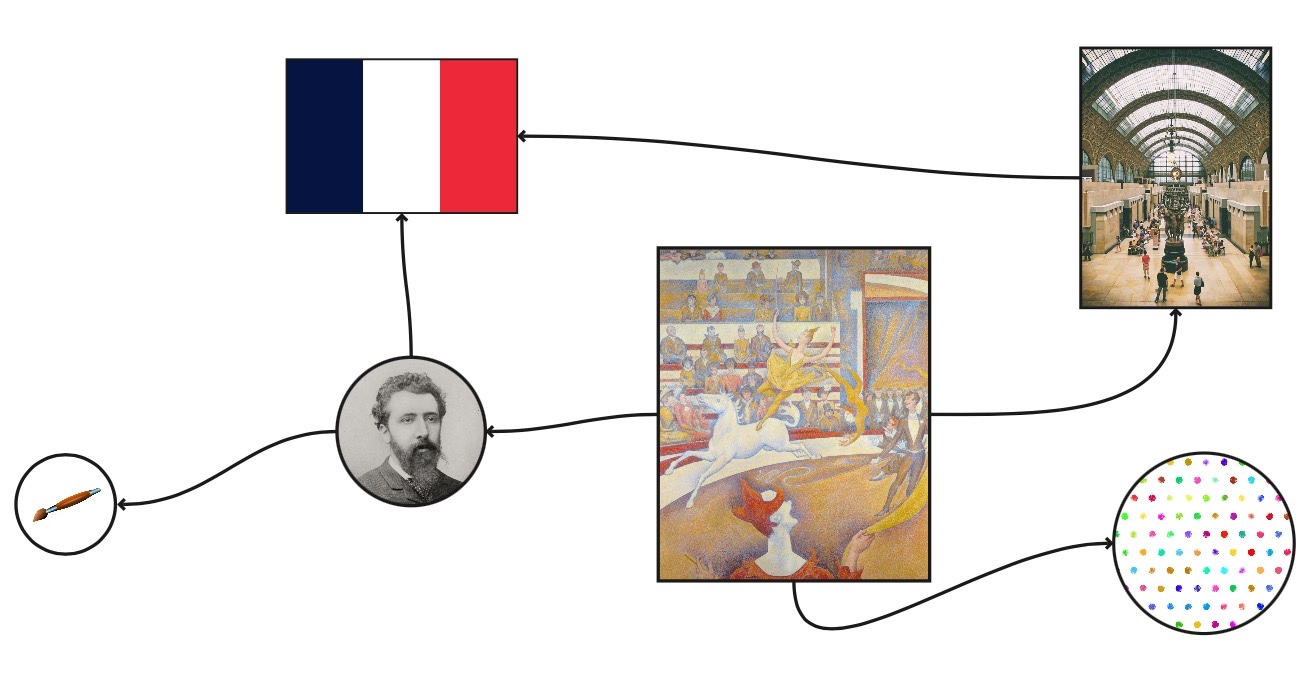
\includegraphics[width=\textwidth]{images/no_linked_data.jpg}
	\caption{Representation of a web of documents without unambiguous indications of what the documents and the links between them represent}
	\label{fig:no_linked_data}
\end{figure}

Simply put, data coming from different sources can be labeled as Linked Data as soon as they are linked by typed links. In other words, links are no longer just an indication of how to reach another document. Indeed, within the Linked Data story, they also contain information about what exactly the link in question represents. Linked Data thereby ensures the meaning of data is explicitly defined, in turn rendering the data machine-readable. Figure~\ref{fig:linked_data} represents the same web of documents as Figure~\ref{fig:no_linked_data}, but this time in accordance with the idea of Linked Data. Indeed, the documents have been given an  unambiguous indication of what they represent, and their mutual semantics have also been clarified thanks to the labeling of their links. \citep{bizer2011linked}

\begin{figure}[htbp]
    \centering
	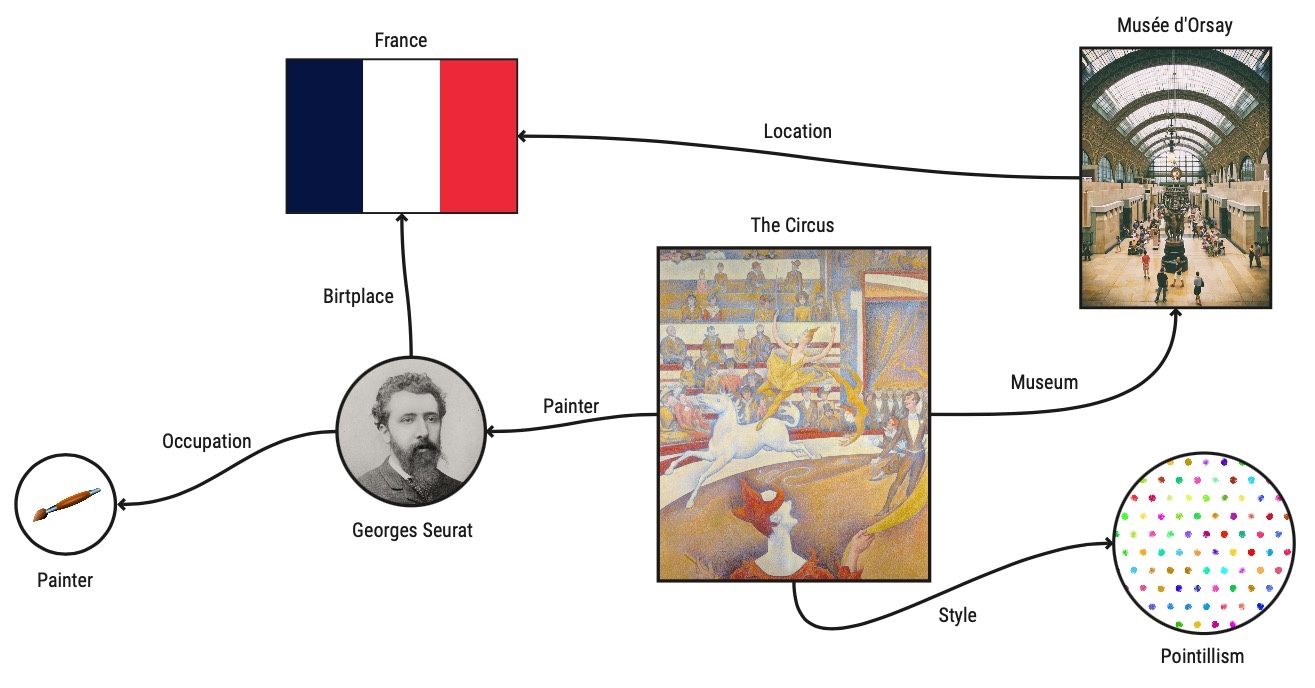
\includegraphics[width=\textwidth]{images/linked_data.jpg}
	\caption{Representation of a web of documents composed according to the spirit of Linked Data}
	\label{fig:linked_data}
\end{figure}

Although several technologies exist to achieve the goals of Linked Data, the use of URIs is essential. After all, since URIs are unique, they can unambiguously reference a particular entity. Practically speaking, the URIs that appear in a Linked Data document can be dereferenced using the HTTP protocol in order to retrieve the underlying entities. For instance, \mintinline{text}{https://stad.gent/id/concept/530010539}, is a URI that can be dereferenced using the HTTP(S) protocol. By dereferencing URI after URI in this way, little by little a - what could be called - \textit{field of information} unfolds, whose semantics can be unambiguously determined by both man and machine. \citep{bizer2011linked}

To clarify the concept of Linked Data, \citet{berners2006linked} put forth four principles to be taken into consideration.
\begin{enumerate}

    \item \textbf{Use URIs as names for things}\\
    The principle of using URIs has already been discussed above.
    
    \item \textbf{Use HTTP URIs so that people can look up those names}\\
    The principle of using the HTTP protocol to dereference URIs was also touched on above. Nevertheless, it is important to reiterate its importance, as there are other protocols besides HTTP for dereferencing URIs. However, these will technically differ from the HTTP protocol, each in its own different ways. For example, not using the ubiquitous Domain Name System (DNS), is, among others, a common practice among alternative protocols. However, in light of clarity and uniformity, as well as for other technical reasons, the HTTP protocol should be adhered to. \citep{berners2006linked}
    
    \item \textbf{When someone looks up a URI, provide useful information, using the standards (RDF, SPARQL)}\\
    Obviously, it would not fit within the spirit of Linked Data to obtain a raw data dump when dereferencing a URI that was included from another document as a \textit{Linked Data link}. The obtained data itself must comply with Linked Data principles. Therefore, there are some standards that clearly indicate how ontologies can be described. Consequently, to enable the construction of applications that deal with Linked Data, it goes without saying that a Linked Data document should be built according to the principles of an existing standard. RDF is the most common such standard and is therefore discussed further in Sections~\ref{subsec:rdf}. In addition, Section~\ref{subsec:sparql} introduces the SPARQL query interface. After all, large datasets are expected to also provide such interface. \citep{berners2006linked}
    
    \item \textbf{Include links to other URIs so that they can discover more things}\\
    The fourth and final principle, too, is rather obvious. After all, by definition, one can only speak of Linked Data when a document refers to at least one other document. In addition, to help advance the cause of transforming the World Wide Web in its current form into a semantic World Wide Web, aided by the concepts of Linked Data, it is preferable to also include links to documents belonging to other sites. \citep{berners2006linked}
    
\end{enumerate}

In conclusion, Linked Data plays a crucial role in giving meaning to the Web by enabling the interconnection and integration of diverse data sources. By adhering to the principles of unique URIs, dereferencing, linking, and using standardized formats, Linked Data fosters a more structured and interconnected web of knowledge. Examples such as DBpedia\footnote{\url{https://www.dbpedia.org}}, which provides a structured representation of Wikipedia data, and Friend of a Friend (FOAF), which allows for the description of people and their relationships, illustrate how publishing data as Linked Data benefits from enhanced data discoverability, interlinking with other datasets, and enabling novel applications and insights. Local initiatives like Collections of Ghent (CoGhent\footnote{\url{https://www.collections.gent}}), which digitizes art collections from cultural houses in Ghent and will be further discussed in Section~\ref{sec:coghent}, similarly demonstrate the potential of Linked Data for local organizations in contributing to the broader web of knowledge. \citep{auer2007dbpedia} \citep{golbeck2008linking} \citep{van2022publishing}

\subsection{Resource Description Framework}
\label{subsec:rdf}

The idea behind Linked Data is interesting in itself, but does not yet describe exactly how to get started with it. Therefore, this section introduces the Recourse Description Framework (RDF). Developed under the auspices of the World Wide Web Consortium (W3C), RDF is an infrastructure that allows for the construction of Linked Data datasets and their metadata. Consequently, this not only allows data publishers to lay out their data as Linked Data, but also gives data consumers clear guidance on how the data can be understood. Note here that data consumers can be both individuals and computer applications. \citep{miller1998introduction}

An interesting way to understand RDF is to first make a jump to the English language. Take the sentence below:
\begin{center}
    \textbf{The birthplace of Georges Seurat is France.}
\end{center}
According to English grammar, the \textit{who} or \textit{what} around which a sentence revolves, is called the subject of the sentence. Therefore, when looking at the sentence above, \textit{Georges Seurat} is its subject. In addition, the part of a sentence that gives more information about the subject, is referred to as the predicate, making \textit{the birthplace} the predicate in the above sentence. Finally, the matching value complementing the predicate and completing the sentence, is also of importance. Logically, in the case of the sentence above, that would be \textit{France}. Together, these three components form the most basic building blocks of a sentence. In fact, no matter their lengths, combined, they will always establish a piece of knowledge, exactly what RDF also seeks to accomplish. \citep{powers2003practical}

The building blocks of RDF data are basically exactly the same as those of linguistic sentences. After all, they are also three in number and even partly share the same names. Moreover, much like with sentences, combined, they form a single yet very clear piece of knowledge. Unlike the English language, however, they are not referred to as sentences. Rather, they are called triples. \citep{powers2003practical}
\begin{itemize}

    \item \textbf{Resource}\\
    \cite{miller1998introduction} defines a resource as any object that is uniquely identifiable by a URI. This enables it to come in different forms: as a web page, as an entire website or simply as any resource on the Web that conveys information in one way or another. \citep{candan2001resource}
    
    To make the comparison with the English language again, in a triple, the resource corresponds to the subject in a sentence. Moreover, in practice, the term \textit{subject} is often preferred over \textit{resource}. \citep{powers2003practical}

    \item \textbf{Property Type}\\
    A property type, or simply a property, introduces a specific aspect, characteristic, attribute, or relationship of a resource. A property type always expects a value to ultimately define the piece of knowledge represented by a triple. \citep{candan2001resource} \citep{miller1998introduction}
    
    As for property types, in practice, the corresponding term from the English language, \textit{predicate}, is also frequently used as opposed to the more theoretical \textit{property type}. \citep{powers2003practical}

    \item \textbf{Value}\\
    A value resolves the concept or relationship initiated by a property type. In this way, it captures the knowledge conveyed by the triple. Values can be represented as text strings, numbers, or any atomic data. However, they can also be resources themselves. This characteristic allows triples therefore to be the building blocks of a web of knowledge. \citep{miller1998introduction}
    
    It is evident that a value in a triple corresponds to a value in an English sentence. However, in practice, the term \textit{object} is often preferred. \citep{powers2003practical}
    
\end{itemize}

While triples convey a clear and distinct piece of knowledge, a collection of triples can naturally convey a more comprehensive knowledge. Such a collection of triples, interconnected by values that are themselves resources, is also referred to as an \textit{RDF description}. Figure~\ref{fig:rdf_description} illustrates what such an RDF description might look like. Additionally, it is important to note that each of its components, whether it be a resource, property type, or value, does not necessarily have to be a digital concept. After all, Web assets can perfectly represent real-life concepts. \citep{miller1998introduction} \citep{candan2001resource}

\begin{figure}[htbp]
    \centering
	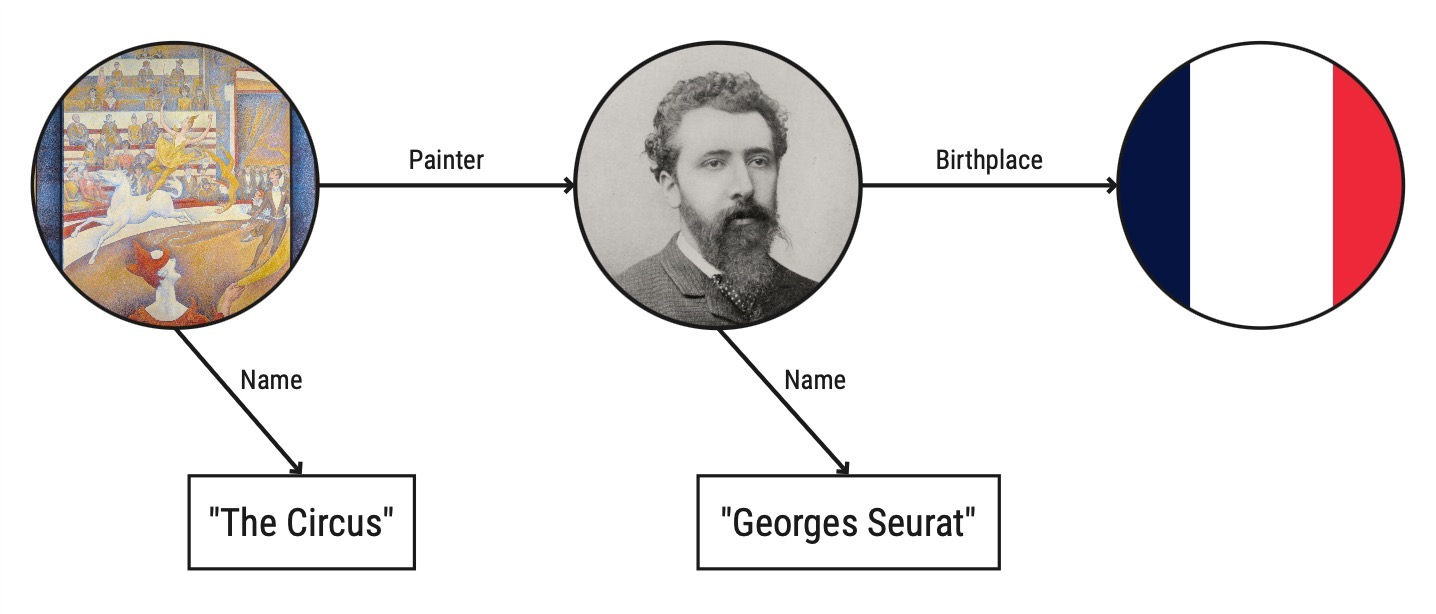
\includegraphics[width=\textwidth]{images/rdf_description.jpg}
	\caption{Representation of an RDF description}
    \caption*{Circles represent resources, arrows represent property types and values are situated at the end of arrows}
	\label{fig:rdf_description}
\end{figure}

Clearly, different terms exist to denote the same RDF concepts. For instance, in addition to the synonyms mentioned above, in literature, the term \textit{statement} is sometimes preferred over \textit{triple}. However, in light of uniformity and clarity, throughout the rest of this text, the terms \textit{triple}, \textit{subject}, \textit{predicate} and \textit{object} will be used instead of their counterparts. \citep{candan2001resource}

\subsection{Resource Description Framework Syntax}
\label{subsec:rdf_syntax}

What constitutes RDF exactly, should be clear by now, but the question of how to actually write down RDF descriptions, still remains to be answered. Therefore, this section introduces some RDF syntaxes. However, since they are not the focus of this research, they will not be discussed in detail. Instead, their outlines will be illustrated by presenting the RDF description from Figure~\ref{fig:rdf_description} in the syntax in question. Incidentally, since the schema presented in Figure~\ref{fig:rdf_description} also has clear guidelines on how to be used, in itself, it also qualifies as an RDF syntax, albeit a graphical one. \citep{miller1998introduction}

All the syntaxes to be discussed are instantiations of the RDF Model and Syntax Specification, providing concrete implementations. However, the first syntax stands apart from the rest as it primarily serves as a notation recommendation for humans to express RDF descriptions in a manner that is unambiguous yet simple. Unlike the other syntaxes, this particular one is not intended for machine consumption. Code Fragment~\ref{lst:human_rdf_syntax} demonstrates how the RDF description, as schematically depicted in Figure~\ref{fig:rdf_description}, can be represented using this human-centric syntax. In this representation, resources are enclosed in straight brackets, while property types are represented by arrows. Furthermore, the representation of values varies depending on their types. As denoted, resources are encapsulated within brackets. However, if the values are atomic in nature, they are simply enclosed in quotation marks. \citep{miller1998introduction}

\begin{listing}[htbp]
    \begin{minted}[samepage,fontsize=\small]{text}
[The Circus] ------name--------> "The Circus"
[The Circus] ------painter-----> [Georges Seurat]
[Georges Seurat] --name--------> "Georges Seurat"
[Georges Seurat] --birthplace--> [France]
    \end{minted}
    \caption{RDF description depicted using a human-centric RDF syntax}
    \label{lst:human_rdf_syntax}
\end{listing}

The example from Code Fragment~\ref{lst:human_rdf_syntax} is easy to read, but at the same time rather confusing. Indeed, certain resource names correspond to certain atomic values. One could of course try to give the resources a more generic name to indicate what exactly the resource in question means. However, that would make little sense given the way the following machine-readable RDF syntaxes refer to resources. After all, they use URIs, allowing for a more clear distinction between resources and atomic values.

\begin{itemize}

    \item \textbf{N-Triples}\\
    Code Fragment~\ref{lst:n_triples_syntax} depicts the representation of the RDF description using N-Triples. In this syntax, each line corresponds to a triple, wherein the subject, predicate, and object are delimited by spaces or tabs. The triple is terminated by a period and a new line character. \citep{seaborne2014rdf}

    \begin{listing}[htbp]
        \begin{minted}[samepage,fontsize=\footnotesize]{turtle}
<http://example.org/The_Circus> <http://example.org/name> "The Circus" .
<http://example.org/The_Circus> <http://example.org/painter> <http://example.org/Georges_Seurat> .
<http://example.org/Georges_Seurat> <http://example.org/name> "Georges Seurat" .
<http://example.org/Georges_Seurat> <http://example.org/birthplace> <http://dbpedia.org/resource/France> .
        \end{minted}
        \caption{RDF description depicted using the N-Triples syntax}
        \label{lst:n_triples_syntax}
    \end{listing}
    
    Furthermore, absolute URIs are employed to denote resources, while atomic values are enclosed within quotation marks. With that in mind, it is important to note that if a value itself contains a quotation mark, it must be properly escaped to ensure correct interpretation. \citep{seaborne2014rdf}

    \item \textbf{N3}\\
    Parsing an RDF description in N-Triples syntax is relatively straightforward for computers, but it can be challenging for humans to comprehend at a glance. The use of absolute URIs in N-Triples can lead to visual clutter and hinder readability. To address this, the N3 syntax builds upon N-Triples by introducing the concept of relative URIs. \citep{seaborne2014rdf}

    In N3, it is possible to specify a base URI by including a \mintinline{text}{@base <URI>} directive at the beginning of the document. When a relative URI is encountered elsewhere in the document, the parser appends it to the specified base URI. This allows for a more concise representation of URIs. \citep{berners2011notation3}

    However, RDF descriptions may contain URIs with different base URIs, making a single base URI insufficient. To overcome this limitation, N3 allows the document to be preceded by one or more \mintinline{text}{@prefix prefix: <URI>} directives. These directives associate prefixes with URIs, and the parser appends any relative URI preceded by a prefix to the corresponding base URI associated with that prefix. This mechanism enables the use of multiple base URIs within the same document and enhances the flexibility and expressiveness of the N3 syntax. Code Fragment~\ref{lst:n3_turtle_syntax} illustrates the use of prefixes for the N3 syntax.  \citep{berners2011notation3}

    \begin{listing}[htbp]
        \begin{minted}[samepage,fontsize=\small]{turtle}
@prefix ex: <http://example.org/> .
@prefix dbp: <http://dbpedia.org/resource/> .

ex:The_Circus ex:name "The Circus" .
ex:The_Circus ex:painter ex:Georges_Seurat .
ex:Georges_Seurat ex:name "Georges Seurat" .
ex:Georges_Seurat ex:birthplace dbp:France .
        \end{minted}
        \caption{RDF description depicted using the N3 and Turtle syntaxes}
        \label{lst:n3_turtle_syntax}
    \end{listing}

    \item \textbf{Turtle}\\
    The Turtle syntax is very similar to N3. In fact, Turtle is a subset of N3. Specifically, Code Fragment~\ref{lst:n3_turtle_syntax} can be processed by a Turtle parser just as well. However, while N3 allows for more expressiveness in principle, Turtle keeps things simpler, making it a popular choice for human readability. \citep{berners2011notation3} \citep{prudhommeaux2014turtle}

    Providing an exhaustive list of the precise differences between the two syntaxes would exceed the scope of this text since the intricacies of RDF syntaxes are not the primary focus here.

    \item  \textbf{RDF/XML}\\
    RDF/XML is one of the earliest RDF syntaxes and remains widely used. To introduce this syntax, Code Fragment~\ref{lst:xml_syntax} serves as a guide.

    \begin{listing}[htbp]
        \begin{minted}[samepage,fontsize=\small]{xml}
<rdf:RDF xmlns:rdf="http://www.w3.org/1999/02/22-rdf-syntax-ns#"
         xmlns:ex="http://example.org/"
         xmlns:dbp="http://dbpedia.org/resource/">
  <rdf:Description rdf:about="http://example.org/The_Circus">
    <ex:name>The Circus</ex:name>
    <ex:painter rdf:resource="http://example.org/Georges_Seurat"/>
  </rdf:Description>
  <rdf:Description rdf:about="http://example.org/Georges_Seurat">
    <ex:name>Georges Seurat</ex:name>
    <ex:birthplace rdf:resource="http://dbpedia.org/resource/France"/>
  </rdf:Description>
</rdf:RDF>
        \end{minted}
        \caption{RDF description depicted using the RDF/XML syntax}
        \label{lst:xml_syntax}
    \end{listing}

    The RDF description in RDF/XML is enclosed within \mintinline{text}{rdf:RDF} elements, where necessary prefixes can also be defined. While an XML declaration like \mintinline{text}{<?xml version="1.0"?>} can precede the RDF/XML document, it is optional and omitted in Code Fragment~\ref{lst:xml_syntax} to focus primarily on the basics of RDF syntaxes. \citep{gandon2014xml}

    Upon encountering the \mintinline{text}{rdf:RDF} tag, a parser recognizes that it should process an RDF description. In RDF/XML, such an RDF description is constructed using one or more \mintinline{text}{rdf:Description} elements. In fact, each \mintinline{text}{rdf:Description} element represents a subject, and its optional \mintinline{text}{rdf:about} attribute denotes the subject's URI. Consequently, the triples associated with the subject are enclosed within the corresponding \mintinline{text}{rdf:Description} tags. Predicates on the one hand, whether represented using a prefix or not, have their own elements. The representation of subjects, on the other hand, depends on their nature: for atomic values, they can simply be placed between opening and closing subject tags, while for resource subjects, their URIs are included as the value of an \mintinline{text}{rdf:resource} attribute within the subject tag. \citep{gandon2014xml}

    Once again, it is important to note that the Code Fragments used in this section provide only an introductory glimpse of the proposed syntaxes. They cover only a small portion of the potential scope of a syntax. Code Fragment~\ref{lst:xml_syntax}, in particular, demonstrates that RDF/XML syntax can obscure simplicity, especially when dealing with more extensive RDF descriptions. Consequently, RDF/XML is not commonly used for human-readable purposes but rather as a syntax primarily intended for machine consumption. \citep{dongo2019srdf}

    \item \textbf{JSON-LD}\\
    The final RDF syntax introduced is called JSON-LD. Similar to RDF/XML, JSON-LD builds upon an existing syntax for representing data on the web. However, JSON-LD representations are generally more human-readable. As most resources and examples in the following text will be presented in JSON-LD, a slightly more comprehensive overview of this syntax is provided compared to the previous ones. Nevertheless, what follows is not an exhaustive listing of all the intricacies of the syntax. Instead, it aims to offer readers a concise introduction to JSON-LD without prior knowledge, making the rest of the text more easily comprehensible. For those seeking more in-depth information about JSON-LD, it is recommended to consult other sources\footnote{The W3C JSON-LD 1.1 Recommendation provides very in-depth information about the JSON-LD syntax: \url{https://www.w3.org/TR/json-ld11/}.}.

    It is evident that the same data can be represented in various ways, and this applies to RDF data as well. While the visual representation of an RDF description, as depicted in Figure~\ref{fig:rdf_description}, is relatively straightforward, converting it into a fully textual format poses certain choices to be made. After all, there are numerous possibilities regarding the exact data representation. In the introduction of previous syntaxes, a specific representation was chosen each time. However, in this section, three different approaches for representing the same set of data using the JSON-LD syntax are presented.

    To start off, Code Fragment~\ref{lst:json_ld_nested_syntax} closely resembles the previous examples, using nesting to store all the data in a single JSON-LD document. However, some may question whether it is appropriate to make the \mintinline{text}{George_Seurat} resource a child of \mintinline{text}{The_Circus} resource, implying a hierarchical relationship that may not be relevant.

    \begin{listing}[htbp]
        \begin{minted}[samepage,fontsize=\small]{jsonld}
{
  "@context": {
    "ex": "http://example.org/",
    "dbp": "http://dbpedia.org/resource/"
  },
  "@id": "ex:The_Circus",
  "ex:name": "The Circus",
  "ex:painter": {
    "@id": "ex:Georges_Seurat",
    "ex:name": "Georges Seurat",
    "ex:birthplace": "dbp:France"
  }
}
        \end{minted}
        \caption{RDF description with nested objects depicted using the JSON-LD syntax}
        \label{lst:json_ld_nested_syntax}
    \end{listing}

    Subsequently, in Code Fragment~\ref{lst:json_ld_spread_syntax}, the data is split into two JSON-LD documents. Utilizing URIs, the documents can still refer to each other uniquely, without suggesting any hierarchical relationship between the resources.

    \begin{listing}[htbp]
        \begin{minted}[samepage,fontsize=\small,escapeinside=||]{jsonld}
|Document 1:|
{
  "@context": {
    "ex": "http://example.org/"
  },
  "@id": "ex:The_Circus",
  "ex:name": "The Circus",
  "ex:painter": "ex:Georges_Seurat"
}

|Document 2:|
{
  "@context": {
    "ex": "http://example.org/",
    "dbp": "http://dbpedia.org/resource/"
  },
  "@id": "ex:Georges_Seurat",
  "ex:name": "Georges Seurat",
  "ex:birthplace": "dbp:France"
}
        \end{minted}
        \caption{RDF description spread over two documents depicted using the JSON-LD syntax}
        \label{lst:json_ld_spread_syntax}
    \end{listing}

    Finally, Code Fragment~\ref{lst:json_ld_graph_syntax} takes a distinct approach by using the \mintinline{text}{@graph} property. This allows listing the necessary resources in a JSON array, placing them on equal footing within a single document. However, this method introduces extra clutter and overhead compared to the previous approaches. \citep{kellogg2020jsonld}

    Ultimately, the choice of representation depends on the specific use case and the desired balance between simplicity and expressiveness. Each approach has its advantages and trade-offs, showcasing the flexibility of the JSON-LD syntax in accommodating different data representation needs.

    \begin{listing}[htbp]
        \begin{minted}[samepage,fontsize=\small]{jsonld}
{
  "@context": {
    "ex": "http://example.org/",
    "dbp": "http://dbpedia.org/resource/"
  },
  "@graph": [
    {
      "@id": "ex:The_Circus",
      "ex:name": "The Circus",
      "ex:painter": {
        "@id": "ex:Georges_Seurat"
      }
    },
    {
      "@id": "ex:Georges_Seurat",
      "ex:name": "Georges Seurat",
      "ex:birthplace": {
        "@id": "dbp:France"
      }
    }
  ]
}
        \end{minted}
        \caption{RDF description as a graph depicted using the JSON-LD syntax}
        \label{lst:json_ld_graph_syntax}
    \end{listing}

    Understanding Code Fragments~\ref{lst:json_ld_nested_syntax}, \ref{lst:json_ld_spread_syntax}, and \ref{lst:json_ld_graph_syntax} becomes relatively straightforward after having discussed the previous syntaxes. However, two aspects deserve further attention: the use of \mintinline{text}{@id} and \mintinline{text}{@context} keywords in JSON-LD.

    Firstly, the \mintinline{text}{@id} keywords uniquely identify the proposed resources using URIs. Indeed, in the given examples, the id's do exactly that. \citep{kellogg2020jsonld}

    Secondly, the \mintinline{text}{@context} keyword plays a crucial role in JSON-LD. It introduces specifics that can be taken for granted in the actual data, reducing the need for repetitive information and cleaning up the actual JSON. While Code Fragments~\ref{lst:json_ld_nested_syntax}, \ref{lst:json_ld_spread_syntax}, and \ref{lst:json_ld_graph_syntax} use the context in a straightforward way by introducing prefixes, in practice, it can do more than that. Essentially, the context maps terms to URIs. These terms can be freely chosen to enhance human readability. \citep{kellogg2020jsonld}

    W3C's JSON-LD Recommendation\footnote{\url{https://www.w3.org/TR/json-ld11/}} offers a valuable example of how the context is typically used, as illustrated in Code Fragment~\ref{lst:json_ld_context}. The provided context clearly indicates that when the key \mintinline{text}{name} appears in the data, it refers to \mintinline{text}{http://schema.org/name}. Similarly, for \mintinline{text}{image} and \mintinline{text}{homepage}, their respective values are \textit{expanded} into objects that hold additional information. The \mintinline{text}{@type} keyword is also used in the example to indicate the type of the final value. In Code Fragment~\ref{lst:json_ld_context}, it shows that the \mintinline{text}{image} and \mintinline{text}{homepage} keys are followed by an \mintinline{text}{@id}, representing unique resources. Moreover, JSON-LD supports various other types, and custom types can be defined to suit specific requirements. \citep{kellogg2020jsonld}

    \begin{listing}[htbp]
        \begin{minted}[samepage,fontsize=\small]{jsonld}
{
  "@context": {
    "name": "http://schema.org/name",
    "image": {
      "@id": "http://schema.org/image",
      "@type": "@id"
    },
    "homepage": {
      "@id": "http://schema.org/url",
      "@type": "@id"
    }
  },
  "name": "Manu Sporny",
  "homepage": "http://manu.sporny.org/",
  "image": "http://manu.sporny.org/images/manu.png"
}
        \end{minted}
        \caption{Example of context use in JSON-LD, proposed by \cite{kellogg2020jsonld}}
        \label{lst:json_ld_context}
    \end{listing}

    To further enhance the cleanliness of a JSON-LD document, one can opt to store the context as a separate resource rather than embedding it directly in the document. Using this approach, the JSON-LD document includes the URI that references the context as the value for the \mintinline{text}{@context} key. Storing the context separately allows for greater modularity and reusability, making it easier to manage and maintain complex JSON-LD documents. The use of separate contexts can significantly improve the organization and readability of JSON-LD data, enhancing its compatibility with RDF and Linked Data principles. \citep{kellogg2020jsonld}

    To finish off this section on JSON-LD, it is interesting to note that when the JSON-LD document presented in Code Fragment~\ref{lst:json_ld_context} is \textit{expanded}, the data takes on its typical RDF form, adhering fully to the Linked Data principles. This expansion, as shown in Code Fragment~\ref{lst:json_ld_expanded}, reveals the underlying structure of the data and its connection to other resources. \citep{kellogg2020jsonld}

    \begin{listing}[htbp]
        \begin{minted}[samepage,fontsize=\small]{jsonld}
[{
  "http://schema.org/name": [{"@value": "Manu Sporny"}],
  "http://schema.org/url": [{ "@id": "http://manu.sporny.org/" }],
  "http://schema.org/image": [{ "@id": "http://manu.sporny.org/images/manu.png" }]
}]
        \end{minted}
        \caption{Example of an expanded JSON-LD document, proposed by \cite{kellogg2020jsonld}}
        \label{lst:json_ld_expanded}
    \end{listing}

    In summary, the \mintinline{text}{@id} and \mintinline{text}{@context} keywords in JSON-LD contribute to the readability, expressiveness, and flexibility of representing RDF data, enabling a more human-friendly approach to data serialization.
    
\end{itemize}

Before concluding this section on RDF syntaxes, it is crucial to reiterate that the explanations provided are not exhaustive. Only a surface-level overview of these syntaxes was covered, and there is much more to explore and learn about them. This section serves as a reference for those with limited or no prior knowledge of RDF syntaxes, aiming to facilitate their understanding of the remaining text. In the following sections, several RDF examples will be presented, with the majority of them using the Turtle and JSON-LD syntaxes. However, there will be no further elaboration on new elements that are specific to each syntax unless they are essential for a clear understanding of the text. For readers seeking a more in-depth understanding of the syntaxes, additional resources are recommended to further explore their intricacies and capabilities.

\subsection{SPARQL}
\label{subsec:sparql}

SPARQL is a set of specifications that describes how to work with RDF data. The latest version of SPARQL is SPARQL \mintinline{text}{1.1}, which, among others, stipulates the workings of an update language, query results formats, and federated querying. But arguably most importantly, it defines the SPARQL query language. \citep{buil2013sparql}

The SPARQL query language is designed for querying RDF data sources. While \mintinline{text}{CONSTRUCT} queries return results as new RDF data, queries with a \mintinline{text}{SELECT} clause return specific data points. This research exclusively focuses on the latter type of queries. \citep{seaborn2013sparql}

The \mintinline{text}{SELECT} clause specifies which variables - in their original form or modified - should be returned as results from the \mintinline{text}{WHERE} clause. The \mintinline{text}{WHERE} clause in turn defines the \textit{basic graph pattern} (BGP) that the datasource(s) need to match. Such a BGP consists of one or more triple patterns that are matched one by one with the triples from the queried dataset(s). Triple patterns are similar to regular triples, but the subject, predicate, and/or object can be replaced with a variable. When a triple pattern matches a triple, each of its variables is combined with the value of the corresponding triple's corresponding element, into a \textit{binding}. In subsequent triple patterns, previously encountered variables can reappear, allowing their corresponding bindings to already narrow down the list of possible matching triples. \citep{seaborn2013sparql}

The \mintinline{text}{SELECT} and \mintinline{text}{WHERE} clauses are essential to SPARQL queries, but SPARQL provides many other keywords to further specify queries. For instance, \mintinline{text}{FILTER} statements can subject variable values to additional tests, wrapping certain triple patterns in an \mintinline{text}{OPTIONAL} clause alleviates them from necessarily being matched, and requesting only unique results can be done using \mintinline{text}{DISTINCT}. More advanced options include merging different result sets using the \mintinline{text}{UNION} keyword, aggregating results with a \mintinline{text}{GROUP BY} statement, and manipulating variable values on the spot using a \mintinline{text}{BIND} form. Basic query necessities like setting a limit (\mintinline{text}{LIMIT}) and an offset (\mintinline{text}{OFFSET}) are also available. Finally, queries can be made more readable and organized by using \mintinline{text}{PREFIX} statements at the top of the query, preventing the need of writing out full URIs. In conclusion, the use and combination of any of these keywords make it possible to craft a wide range of queries. The queries presented throughout this research can generally be considered \textit{simple} and should therefore be comprehensible to readers who are new to the subject. However, for those interested, Section~\ref{sec:coghent_example_queries} already provides some example queries to explore. \citep{seaborn2013sparql} \citep{ducharme2013learning}

Up to this point, the terms \textit{triple} and \textit{triple pattern} have been used exclusively. However, it is important to note that in literature, the terms \textit{quad} and \textit{quad pattern} also often appear. Essentially, quads are the same as triples but they introduce a fourth element, namely a \textit{named graph}. In fact, these named graphs \textit{group} certain triples and allow datasets to be subdivided further. This research does not further discuss nor employ named graphs, yet since the term \textit{quad} is more specific, from this point onward, it will be used in favor of the term \textit{triple}. \citep{taelman2020quad}

\section{Link-Traversal-based Query Processing}
\label{sec:ltqp}

The vision behind Linked Data is a compelling one: a web of interconnected data that can be seamlessly queried and navigated. However, the practicalities of querying this vast, decentralized network using tools like SPARQL over RDF representations present challenges. How does one effectively access and integrate data scattered across diverse sources? This is where \textit{Link Traversal-based Query Processing} (LTQP) - often simply referred to using the \textit{broader} term \textit{link traversal} - becomes indispensable. By dynamically traversing links between documents, LTQP offers a solution that is not confined to a static dataset but instead capitalizes on the web's inherent interconnectivity. Through this method, the promise of Linked Data moves a step closer to its practical realization in a decentralized web environment. In Section~\ref{subsec:lt_basics}, a deeper dive into the foundational mechanisms of link traversal is presented, leading to Section~\ref{subsec:reachability_criteria} exploring possible criteria that determine which links should be pursued during the query process. \citep{hartig2012foundations} \citep{taelman2023ltqp}

\subsection{Link Traversal Basics}
\label{subsec:lt_basics}

Whereas \textit{conventional} SPARQL query processing is confined to the scope of the predetermined dataset(s), link traversal can, in principle, involve the entire RDF web in the query process by following the URIs - links - between RDF documents. The querying dataset is, in other words, dynamically expanded. To discuss this link traversal query process, the documents depicted in Code Fragment~\ref{lst:json_ld_spread_syntax} are used. The query engine is instructed to find the birthplace of the painter of the painting \textit{The Circus}, but initially only receives the URI to the first document. The specific query is shown in Code Fragment~\ref{lst:sparql_spread}.
\begin{enumerate}
    \item \textbf{Initialization}\\
    The process starts with a link queue populated with seed URIs, either user-defined or derived from the query. For this example, the seed URI is derived from the query and points to the document containing the \textit{The Circus} painting's resource.
    \item \textbf{Iteration and Appending}\\
    During the iteration process, the link at the head of the queue is accessed, leading to the associated document. All URIs from that document are then added back into the queue. In this example, after accessing the document with the \textit{The Circus} resource, the link associated with the \textit{Georges Seurat} resource leads to the second document in Code Fragment~\ref{lst:json_ld_spread_syntax}. Furthermore, during this process, the \mintinline{text}{http://dbpedia.org/resource/France} link would also be added to the link queue. From this resource's document, other links might be discovered and added to the queue, and so on.
    \item \textbf{Query Execution}\\
    The query runs over the union of all the RDF triples from the discovered documents. For this example, this results in identifying \textit{France} as the birthplace of the painter of \textit{The Circus}.
\end{enumerate}
\citep{taelman2023ltqp}

\begin{listing}[htbp]
    \begin{minted}[fontsize=\small]{sparql}
PREFIX ex:<http://example.org/>

SELECT ?birthplace

WHERE {
  ex:The_Circus ex:painter ?painter.
  ?painter ex:birthplace ?birthplace.
}
    \end{minted}
    \caption{SPARQL query querying data that is spread over the two documents displayed in Code Fragment~\ref{lst:json_ld_spread_syntax}}
    \label{lst:sparql_spread}
\end{listing}

It is important to note that link traversal is theoretically an infinite process. As links lead to more documents, which in turn contain more links, the process can continue indefinitely. This is also apparent from the example. Indeed, during the iteration process, it is very likely the query engine would have had to follow an enormous - possibly infinite - collection of links, as the \mintinline{text}{http://dbpedia.org/resource/France} resource might introduce other links, which in turn might introduce other links as well, and so on. This highlights the importance of introducing criteria to determine which links should be pursued and which should be ignored, ensuring more efficient query processing. \citep{taelman2023ltqp} \citep{hartig2012foundations}

\subsection{Reachability Criteria}
\label{subsec:reachability_criteria}

In LTQP, determining which links to traverse is essential. \citet{hartig2012foundations} introduced the concept of \textit{reachability criteria} to guide this decision-making process:
\begin{itemize}
    \item \textbf{\textit{cAll}}\\
    This criterion represents the most unrestricted approach to link traversal. It allows for arbitrary paths to reach Linked Data documents by following every possible link without any constraints. This approach adheres to the most basic idea of link traversal, ensuring comprehensive data retrieval but potentially leading to information overload.
    
    \item \textbf{\textit{cNone}}\\
    This is the exact opposite of \textit{cAll}. It is the most restrictive criterion, where no links are pursued at all. Effectively, link traversal is disallowed, confining the process strictly to the initial document.
    
    \item \textbf{\textit{cMatch}}\\
    This criterion is based on \textit{query pattern-based reachability}. Specifically, a link is pursued only if the quad it is part of corresponds to a specific quad pattern in the executed query. This approach offers a more targeted traversal, ensuring that only relevant links corresponding to the query patterns are followed.
\end{itemize}
\citep{hartig2012foundations}

While these criteria provide foundational strategies for traversal, they represent theoretical approaches. In practice, the actual traversal might be influenced by various factors, and more intricate rules can be devised to steer an LTQP engine. In the section that follows, namely Section~\ref{sec:comunica}, a system is introduced that allows for easy configuration of custom SPARQL query engines - link traversal engines as well - in turn allowing for the practical implementation of the aforementioned link traversal strategies, as well as new ones.

\section{Comunica}
\label{sec:comunica}

While various solutions exist for querying RDF data using SPARQL, Comunica\footnote{\url{https://comunica.dev}} stands out for several reasons. Beyond its capability to support heterogeneous interfaces, allowing for seamless querying across diverse data sources like data dumps, RDF documents, SPARQL endpoints and Triple Pattern Fragments (TPF) interfaces, it is built on and using web-based technologies. This ensures broad compatibility and easy integration with browsers and web applications. However, Comunica's defining characteristic is arguably its modularity. Users can choose from existing configurations or craft custom ones, creating query engines tailored to specific needs. The technical foundations that enable this modular approach are elaborated upon in Section~\ref{subsec:comunica_building_blocks}. \citep{taelman2018comunica}

\subsection{Building Blocks}
\label{subsec:comunica_building_blocks}

Comunica's unique modularity is achieved through an architectural design in which three types of components are core.
\begin{itemize}
    \item \textbf{Actors}\\
    Actors are the primary computational units in Comunica. They are responsible for processing specific messages they receive via the buses they are subscribed to. Each actor is designed to accept certain types of messages and respond accordingly, ensuring efficient and targeted processing.

    \item \textbf{Buses}\\
    Buses serve as communication channels in Comunica. They facilitate the interaction between actors and mediators. To optimize performance and prevent congestion, Comunica employs multiple buses, each catering to different types of messages. This separation ensures that each bus handles specific tasks, streamlining the communication process.

    \item \textbf{Mediators}\\
    Mediators play a pivotal role in determining the best actor for a given task. They are connected to a single bus and operate in two phases: the test phase and the run phase. Initially, in the test phase, mediators evaluate the conditions under which each actor on the bus can perform a task. Once the most suitable actor is identified, the run phase is initiated, where the chosen actor processes the message and returns the result.
\end{itemize}
\citep{taelman2018comunica}

Comunica is not only modular, but it also boasts a highly adaptable interface thank to its integration with \textit{Component.js}, a dependency injection framework. This framework allows for the semantic description of Comunica components in JSON-LD format, facilitating the dynamic selection and combination of components based on configuration files. As a result, Comunica can serve diverse purposes, from executing SPARQL queries to custom RDF parsing. The platform already offers a wide range of modules\footnote{\url{https://github.com/comunica/comunica/tree/master/packages}}, including buses, mediator types, and actors. Moreover, while it also already offers predetermined engine configurations\footnote{\url{https://github.com/comunica/comunica/tree/master/engines}} that combine these modules, users are also empowered to craft their own configurations, tailoring engines to their specific needs. \citep{taelman2018comunica}

\subsection{Link Traversal Engines}

A review of the Comunica GitHub repository\footnote{\url{https://github.com/comunica/comunica}} reveals a comprehensive set of modules and configurations. Many of these modules serve to establish Comunica as a proficient \textit{standard} query engine. However, a distinct subset is dedicated to enhancing the engine with LTQP capabilities, and these components are systematically organized in a separate GitHub monorepo\footnote{\url{https://github.com/comunica/comunica-feature-link-traversal}}.

Central to this repository are various link extractors, which determine which links the engine should add to its link queue, effectively defining its \textit{reachability criteria}. For instance, the \textit{All Extract Links Actor}\footnote{\url{https://github.com/comunica/comunica-feature-link-traversal/tree/master/packages/actor-extract-links-all}} and the \textit{Quad Pattern Query Extract Links Actor}\footnote{\url{https://github.com/comunica/comunica-feature-link-traversal/tree/master/packages/actor-extract-links-quad-pattern-query}} are two actors that implement the \textit{cAll} and \textit{cMatch} reachability criteria that were introduced in Section~\ref{subsec:reachability_criteria}. Furthermore, the repository includes additional methodologies. Actors such as the \textit{Predicates Extract Links Actor}\footnote{\url{https://github.com/comunica/comunica-feature-link-traversal/tree/master/packages/actor-extract-links-predicates}} and the \textit{Tree Extract Links Actor}\footnote{\url{https://github.com/comunica/comunica-feature-link-traversal/tree/master/packages/actor-extract-links-extract-tree}} introduce strategies that were not discussed. Specifically, the former instructs the query engine to solely follow links from quads that align with a series of given predicate rules, while the latter ensures the traversal of links that typically appear in documents that follow the TREE specification - this specification will be briefly mentioned in Section~\ref{subsec:ldes}. \citep{taelman2019lt}

In summary, Comunica's modular and adaptable design allows for diverse and profound capabilities in LTQP within the Linked Data landscape.

\section{Collections of Ghent}
\label{sec:coghent}

This research mainly focuses on the data of \textit{Collections of Ghent}\footnote{\url{https://www.collections.gent}} (CoGhent), or \textit{Collectie van de Gentenaar}\footnote{\url{https://www.collectie.gent}} (CoGent) in Dutch. CoGhent is a collaborative effort involving the city of Ghent, Design Museum Gent, Digipolis, and other local organizations in Ghent. CoGhent was established with the aim of collecting and digitizing the city's cultural heritage into a central collection. This collection serves not only as an archive but also as an interactive platform. Residents of Ghent are encouraged to contribute their own heritage stories and objects, creating a vibrant blend of official history and personal narratives within the collection. \citep{leemputten2022gent} \citep{schouppe2022gent}

However, more important for this research is the data specifically published by the participating cultural institutions. These institutions include Design Museum Gent (DMG), Huis van Alijn (HVA), Industriemuseum, STAM, and Archief Gent. Like many other cultural institutions, they use a content management system (CMS) to manage their data. However, to make their data interoperable and open, CoGhent decided to build \textit{Linked Data Event Stream} (LDES) endpoints on top of these systems. \citep{floreverk2022coghent} \citep{van2022publishing}

Before delving deeper into these LDESs, it should be noted that the CoGhent partnership was terminated in June 2023 due to the discontinuation of project funding. However, the infrastructure remains up and running, allowing working with the data to continue. \textit{This information was obtained through personal email correspondence with Olivier Van D'huynslager, Strategic Project Manager and Content Lead at CoGhent.}

\subsection{Linked Data Event Streams}
\label{subsec:ldes}

The CoGhent data, being hosted in LDES, inherently adopts the RDF format, positioning the data within the web of Linked Data. An LDES is characterized by its collection of immutable objects, with each object being represented by RDF triples. This immutability is crucial, signifying that once an object is added to the LDES, it remains unchanged. Instead of updating existing objects, new versions are introduced. The LDES specification provides guidelines on versioning, enabling data consumers to differentiate between various versions of the same object. Furthermore, the inherent immutability suggests that objects are not to be deleted by default. Only when the LDES specifies a particular retention policy (or a combination of them), is the server allowed to delete objects. \citep{colpaert2023ldes}

LDESs are highly suitable for involving rapidly growing and evolving datasets in the Linked Data web. However, even when speed is not the primary concern, LDESs are a great option for publishing collections of equivalent objects. For sure, this is the case with the CoGhent LDESs. Additionally, LDESs can become quite large. Therefore, they are fragmented into different pages. To describe this technically, LDESs rely on the \textit{TREE} specification. The TREE specification allows various relationships between HTTP resources to be defined. As the name suggests, this can even establish very complex \textit{tree-like} structures. To put it simply, all resources belong to the same \mintinline{text}{tree:Collection} but are divided into different \mintinline{text}{tree:Node}s. These nodes are then linked together in specific ways using \mintinline{text}{tree:Relation}s. These relations can describe various types of relationships, but in the case of LDESs, the different \mintinline{text}{tree:Node}s - pages - are simply interconnected in a two-dimensional manner using \mintinline{text}{tree:LessThanRelation}s and \mintinline{text}{tree:GreaterThanRelation}s. The pages' timestamps ultimately help these two types of relations in arrangin the pages from \textit{newest} to \textit{oldest}. \citep{colpaert2023ldes} \citep{colpaert2023tree}

\subsection{Human-Made Objects}

CoGhent's LDESs, specifically, consist of various \textit{Human-Made Object}s (HMO). These HMOs represent tangible and intangible items crafted or influenced by humans, ranging from artworks, books, and monuments to traditions, crafts, and the ideas they convey. The \textit{Open Standaarden voor Linkende Organisaties} (OSLO) initiative plays a pivotal role in standardizing the way they are described and exchanged. Essentially, OSLO is a framework set by the Flemish government to ensure a uniform method of data exchange. In addition, as is the case with all OSLO's standards, HMOs align with international standards to ensure semantic interoperability and a consistent approach to data representation within the cultural heritage domain. Throughout the rest of this research, Human-Made Objects (HMOs) will be predominantly equated with \textit{artworks} for the sake of simplicity. Nonetheless, it is imperative to underscore that this terminology is a notable simplification, as the term \textit{Human-Made Object} encompasses a broad spectrum of items beyond just artworks. \citep{van2022publishing} \citep{vanderperren2021oslo} \citep{linden2021object}

\subsection{Example Queries}
\label{sec:coghent_example_queries}

On its documentation website\footnote{\url{https://coghent.github.io}}, \citet{floreverk2022queries} provides some examples of queries that can be used to query their LDESs. Three of them are discussed here because they not only offer an initial insight into the type of data present in the LDESs but also potentially highlight challenges.

The first example is presented in Code Fragment~\ref{lst:coghent_example_titles} and is very straightforward. Initially, it retrieves all titles of Human-Made Objects. However, they are immediately filtered in order to make sure only those titles containing the word \textit{Gent} are ultimately returned. \citep{floreverk2022queries}

\begin{listing}[htbp]
    \begin{minted}[fontsize=\small]{sparql}
PREFIX cidoc: <http://www.cidoc-crm.org/cidoc-crm/>

SELECT ?title

WHERE { 
  ?object cidoc:P102_has_title ?title.
  FILTER (regex(?title, "Gent", "i"))
}
    \end{minted}
    \caption{SPARQL query fetching Human-Made Objects' titles containing \textit{Gent} as proposed by \citet{floreverk2022queries}}
    \label{lst:coghent_example_titles}
\end{listing}

The second example is depicted in Code Fragment~\ref{lst:coghent_example_labels} and is not much more complex. This time, it retrieves each Human-Made Object's \textit{objectname}'s label. It is worth noting that the \textit{objectname} essentially represents a resource URI pointing to an external vocabulary resource. However, for each \textit{objectname}, the LDESs themselves also specify a \textit{preferred} label, which is an atomic value. In fact, these are the values the query is looking for. \citep{floreverk2022queries}

\begin{listing}[htbp]
    \begin{minted}[fontsize=\small]{sparql}
PREFIX cidoc: <http://www.cidoc-crm.org/cidoc-crm/>
PREFIX skos: <http://www.w3.org/2004/02/skos/core#>

SELECT ?label 

WHERE { 
  ?object cidoc:P41i_was_classified_by ?identifier.
  ?identifier cidoc:P42_assigned ?objectname.
  ?objectname skos:prefLabel ?label
}
    \end{minted}
    \caption{SPARQL query fetching Human-Made Objects' \textit{objectname}'s titles as proposed by \citet{floreverk2022queries}}
    \label{lst:coghent_example_labels}
\end{listing}

Interestingly, a \textit{regular} query engine that only has access to one or more of the CoGhent LDESs can retrieve nothing more than these preferred labels. This is rather unfortunate however, as the vocabulary resource represented by the \textit{objectname} contains much more additional information, including labels in different languages. Still, this additional information can in fact be accessed using a link traversal-capable query engine. Since this is more intricate than it sounds, this is one of the topics covered later on in this research.

The third and final query is shown in Code Fragment~\ref{lst:coghent_example_ordered} and highlights a significant challenge that arises when querying LDESs. After all, it is quite reasonable to assume that users would want to retrieve only the latest version of LDES objects. Code Fragment~\ref{lst:coghent_example_ordered} demonstrates how this can be achieved in query form by cleverly utilizing a nested \mintinline{text}{WHERE} clause, along with the \mintinline{text}{ORDER BY} and \mintinline{text}{DISTINCT} keywords. However, aside from arguably overcomplicating the query, this approach also results in the delivery of results at the absolute end of query execution. After all, the results can only be sorted once they are all available. For this reason, this method cannot be considered optimal for achieving the desired outcome. Again, a different approach is suggested later on in the research, albeit it briefly. \citep{floreverk2022queries}

\begin{listing}[htbp]
    \begin{minted}[fontsize=\small]{sparql}
PREFIX purl: <http://purl.org/dc/terms/>

SELECT DISTINCT ?priref

WHERE {
    SELECT ?object ?priref
    
    WHERE { 
        ?object purl:isVersionOf ?priref.
    }
    
    ORDER BY DESC(?object)
}
    \end{minted}
    \caption{SPARQL query fetching ordered unique versions of all Human-Made Objects as proposed by \citet{floreverk2022queries}}
    \label{lst:coghent_example_ordered}
\end{listing}

\subsection{Query Builder}
\label{subsec:coghent_query_builder}

This research is primarily centered on simplifying the query construction process, especially for culture enthusiasts who may not possess a technical background. In line with this objective, it is pertinent to introduce the \textit{CoGhent Query Builder}\footnote{\url{http://collectievandegentenaar.pythonanywhere.com/querybuilder}}, a user-friendly web application designed with the same goal in mind. As depicted in Figure~\ref{fig:og_query_builder}, the application allows users to select various \textit{properties} and even filter them based on specific string values. These properties, in essence, represent specific data points associated with Human-Made Objects. However, accessing these often involves navigating through a series of predicates. The CoGhent Query Builder simplifies this process by presenting them as a singular property. For a clearer understanding, Code Fragment~\ref{lst:coghent_builder_original} showcases the query generated when the selections illustrated in Figure~\ref{fig:og_query_builder} are made.

\begin{figure}[htbp]
    \centering
	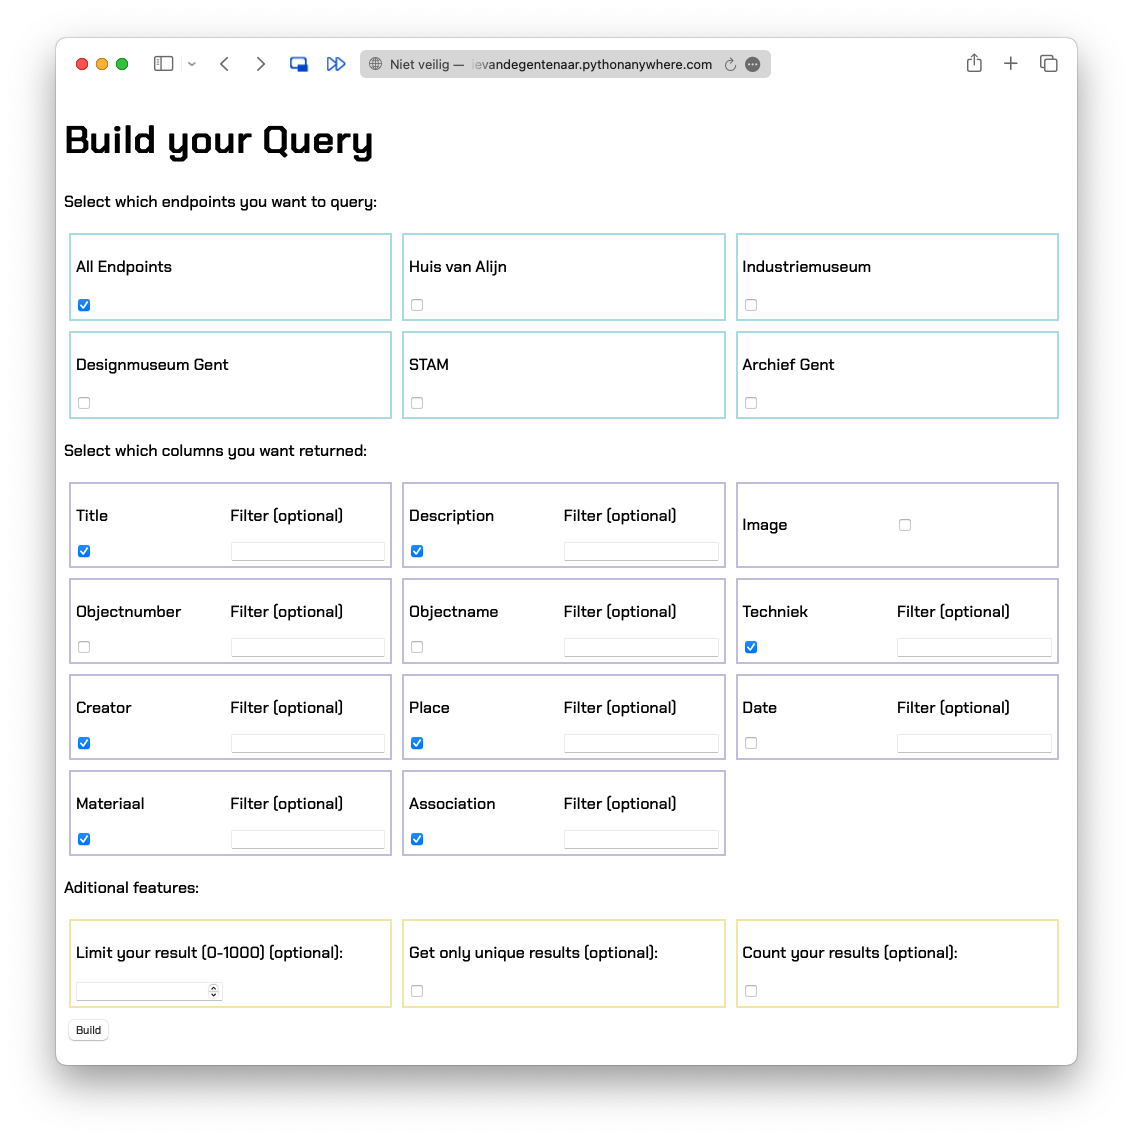
\includegraphics[width=\textwidth]{images/og_query_builder.png}
	\caption{Screenshot of CoGhent Query Builder}
	\label{fig:og_query_builder}
\end{figure}

\begin{listing}[htbp]
    \begin{minted}[fontsize=\small]{sparql}
PREFIX cidoc:<http://www.cidoc-crm.org/cidoc-crm/>
PREFIX adms:<http://www.w3.org/ns/adms#>
PREFIX skos:<http://www.w3.org/2004/02/skos/core#>
PREFIX la:<https://linked.art/ns/terms/>

SELECT ?title ?note ?associatie ?creator ?plaats ?techniek ?materiaal

WHERE {
    # Title
    ?o cidoc:P102_has_title ?title.
    
    # Description
    ?o cidoc:P3_has_note ?note.
    
    # Association
    ?o cidoc:P128_carries ?carries.
    ?carries cidoc:P129_is_about ?about.
    ?about cidoc:P2_has_type ?type.
    ?type skos:prefLabel ?associatie.
    
    # Creator
    ?o cidoc:P108i_was_produced_by ?production.
    ?production cidoc:P14_carried_out_by ?producer.
    ?producer la:equivalent ?equivalent.
    ?equivalent rdfs:label ?creator.
    
    # Place
    ?o cidoc:P108i_was_produced_by ?produced.
    ?produced cidoc:P7_took_place_at ?tookplace.
    ?tookplace la:equivalent ?plaatsequivalent.
    ?plaatsequivalent skos:prefLabel ?plaats.
    
    # Technique
    ?o cidoc:P108i_was_produced_by ?produced.
    ?produced cidoc:P32_used_general_technique ?technique.
    ?technique cidoc:P2_has_type ?hastype.
    ?hastype skos:prefLabel ?techniek.
    
    # Material
    ?o cidoc:P45_consists_of ?consists.
    ?consists cidoc:P2_has_type ?materiaaltype.
    ?materiaaltype skos:prefLabel ?materiaal.
}
    \end{minted}
    \caption{Example of SPARQL query created by original CoGhent Query Builder}
    \label{lst:coghent_builder_original}
\end{listing}

Furthermore, the application provides additional features to enhance the user experience. In concrete terms, users have the flexibility to choose which cultural collection(s) they wish to query, decide if the results should be unique or counted, and even set a limit on the number of results. With its intuitive user interface and these functionalities, the CoGhent Query Builder stands out as a valuable tool for those new to query creation.

\section{International Image Interoperability Framework}
\label{sec:iiif}

In Section~\ref{sec:coghent_example_queries}, only query examples were provided that focus solely on textual data. Within the context of digital art collections, however, this is certainly not sufficient. After all, their most important information is arguably visual in nature. However, visual information typically encompasses more than just an image; often, metadata such as dimensions, notes, and legal information are equally important. In the case of CoGhent, it was decided not to directly include this rather \textit{technical} information in the LDESs. Instead, each CoGhent Human-Made Object refers to an IIIF Manifest. These are fully-fledged RDF resources specifically used to group this kind of information. Their specification is determined by the \textit{International Image Interoperability Framework} (IIIF), an organization described by \citet{snydman2015international} as \textit{a community of academic and national libraries, research institutions, museums, archives, nonprofits and commercial organizations that are committed to interoperable image delivery on the web}. \citep{floreverk2022coghent} \citep{snydman2015international}

\subsection{IIIF Manifests}

IIIF Manifests are central structured documents within the IIIF framework. They provide the overall description of the structure and properties of the digital representation of an object. Each manifest describes how to present a single object, such as a book, photograph, or statue, and carries essential information needed for a viewer to present the digitized content to the user, such as a title and other descriptive details about the object or the intellectual work it represents. \citep{appleby2017presentation}

The structure of IIIF Manifests is stipulated by the \textit{IIIF Presentation API}. However, multiple versions of this API exist. Figure~\ref{fig:pres_api_2} and the following overview briefly introduce the components that are puth forth by Presentation API \mintinline{text}{2.1.1}, as described by \citet{appleby2017presentation}:
\begin{itemize}
    \item \textbf{Sequence}\\
    Defines the order of the views of the object. Multiple sequences can account for situations where there are various valid orders through the content.
    \item \textbf{Canvas}\\
    A virtual container representing a page or view. It provides a frame of reference for content layout.
    \item \textbf{Annotation}\\
    Content resources and commentary are linked to a canvas via annotations.
    \item \textbf{AnnotationList}\\
    An ordered list of annotations, typically linked to a single canvas.
    \item \textbf{Layer}\\
    An ordered list of annotation lists, allowing for higher-level groupings of annotations.
    \item \textbf{Range}\\
    Groups canvases or parts thereof in an ordered list. This can be for textual reasons or physical features.
    \item \textbf{Collection}\\
    An ordered list of manifests or further collections, allowing hierarchical structuring and advertising of manifests.
\end{itemize}

\begin{figure}[htbp]
    \centering
	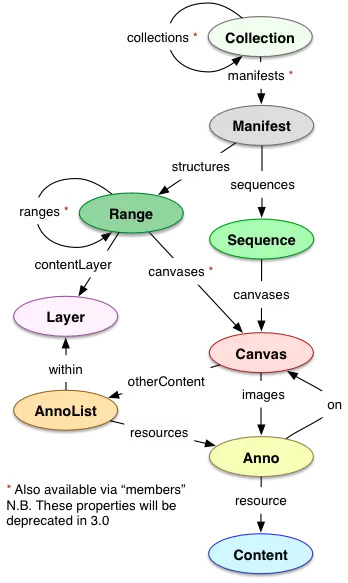
\includegraphics[height=0.6\textheight]{images/pres_api_2.jpg}
	\caption{Presentation API \mintinline{text}{2.1.1}'s resource types visualization taken from \citet{appleby2017presentation}}
	\label{fig:pres_api_2}
\end{figure}

Beyond the Presentation API, IIIF also offers the \textit{Image API}, which delivers the pixels of an image through a structure specifying the image's source, region, size, rotation, quality, and format. This API simply brings the pixels, specifying the image's source, region, size, rotation, quality, and format. The Presentation API then provides just enough metadata to drive a remote viewing experience. \citep{emanuel2018stitching}

To accomodate each Human-Made Object's technical image data, CoGhent specifically relies on Presentation API \mintinline{text}{2.*}. In fact, since each Human-Made Object only has one image, its corresponding IIIF Manifest is structured in a very straightforward manner. Namely, each CoGhent manifest holds one sequence, which in turn holds one canvas, which in turn holds one annotation to house the image resource and its metadata. This structure broadly corresponds to the structure visualized in Figure~\ref{fig:pres_api_2_simple}. \citep{floreverk2022coghent}

\begin{figure}[htbp]
    \centering
	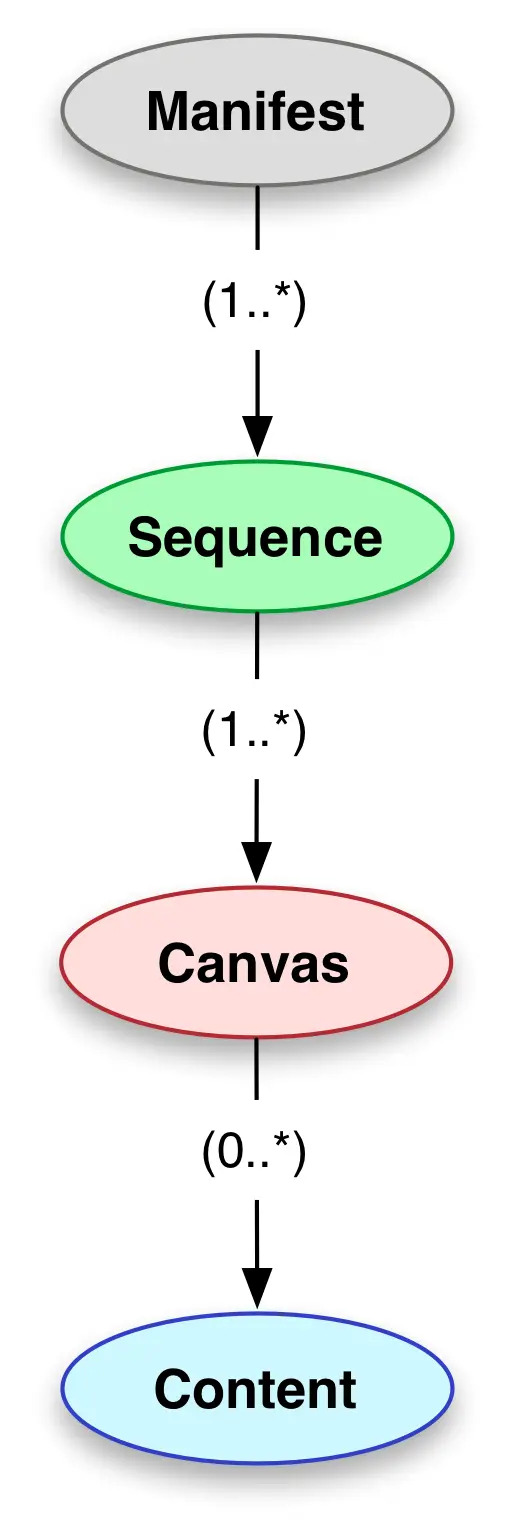
\includegraphics[height=0.4\textheight]{images/pres_api_2_simple.jpg}
	\caption{Presentation API \mintinline{text}{2.1.1}'s \textbf{primary} resource types visualization taken from \citet{appleby2017presentation}}
	\label{fig:pres_api_2_simple}
\end{figure}

Despite the CoGhent manifests relying on Presentation API \mintinline{text}{2.*}, there is in fact a newer version availble, namely Presentation API \mintinline{text}{3.0}. For the sake of completeness, Figure~\ref{fig:pres_api_3} visualizes its components, with the following overview briefly introducing the most notable updates, as described by \citet{appleby2020presentation}:
\begin{itemize}
    \item \textbf{Canvas}\\
    The concept has been expanded to provide a frame of reference for content layout, both spatially and temporally.
    \item \textbf{Annotation Page}\\
    Introduced as an ordered list of Annotations typically associated with a Canvas. Annotation Pages collect and order lists of Annotations.
    \item \textbf{Annotation Collection}\\
    A new concept introduced as an ordered list of Annotation Pages, allowing for higher-level groupings of Annotations.
    \item \textbf{Content}\\
    Defined as web resources, such as images or texts, associated with a Canvas via an Annotation.
\end{itemize}

\begin{figure}[htbp]
    \centering
	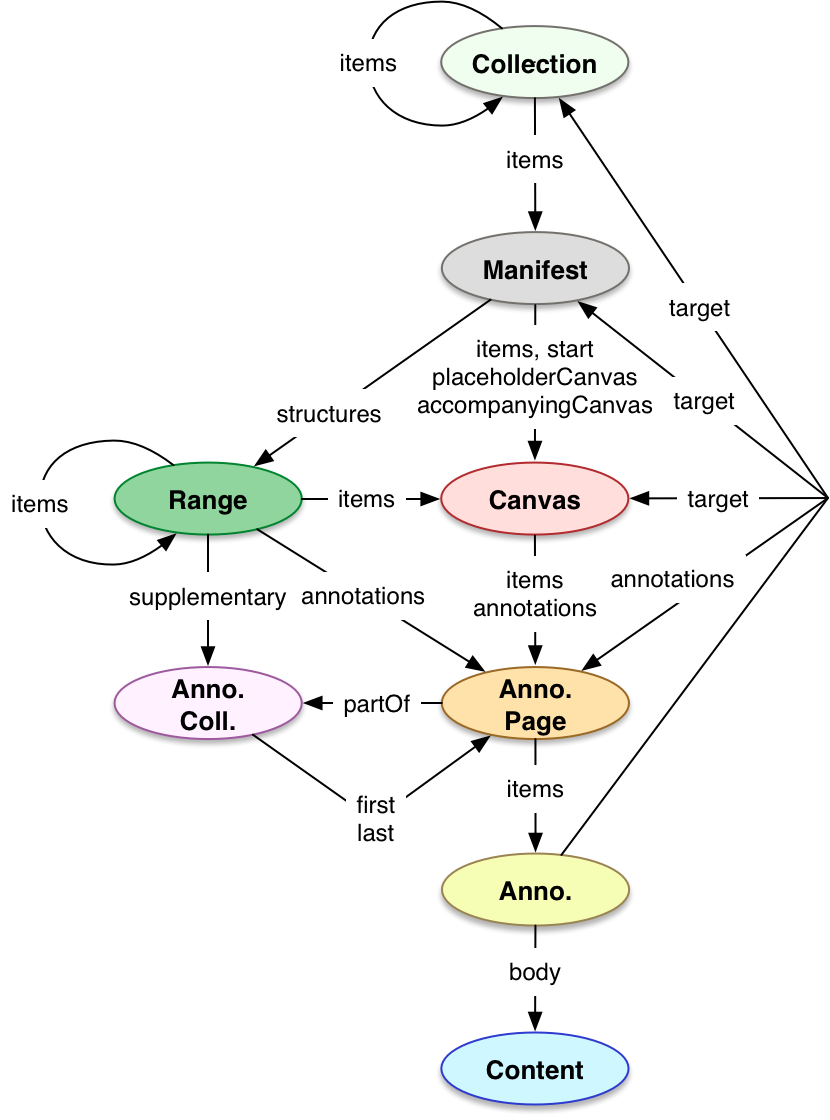
\includegraphics[height=0.6\textheight]{images/pres_api_3.png}
	\caption{Presentation API \mintinline{text}{3.0}'s \textbf{primary} resource types visualization taken from \citet{appleby2020presentation}}
	\label{fig:pres_api_3}
\end{figure}

Whatever the Presentation API version, together with the Image API, it provides a cohesive framework for the representation and delivery of digital images across various platforms and institutions. In fact, it allows for easy visualization using a IIIF Viewer. \citep{snydman2015international}

\subsection{IIIF Viewers}

IIIF Manifests are not only invaluable tools for archiving but also play a pivotal role in visualization. After all, these manifests, which describe the structure and properties of digital representations, provide essential instructions for visualization. In this context, a variety of \textit{IIIF Viewer}s\footnote{IIIF maintains a useful overview of some prominent IIIF Viewers: \url{https://github.com/IIIF/awesome-iiif\#iiif-viewers}} are available that ingest a IIIF Manifest resource and visualize its contents in user-friendly ways. Harnessing the IIIF framework, these viewers ensure consistent features such as multi-image object rendering, pan, deep zoom, and annotation across different platforms. Among the array of IIIF-compatible viewers, \textit{Mirador} stands out. Developed collaboratively by multiple institutions, Mirador exemplifies the capabilities of a viewer built on the IIIF framework, offering users a seamless and interoperable viewing experience. Figure~\ref{fig:mirador} displays a screenshot of the Mirador web app in action. \citep{snydman2015international}

\begin{figure}[htbp]
    \centering
	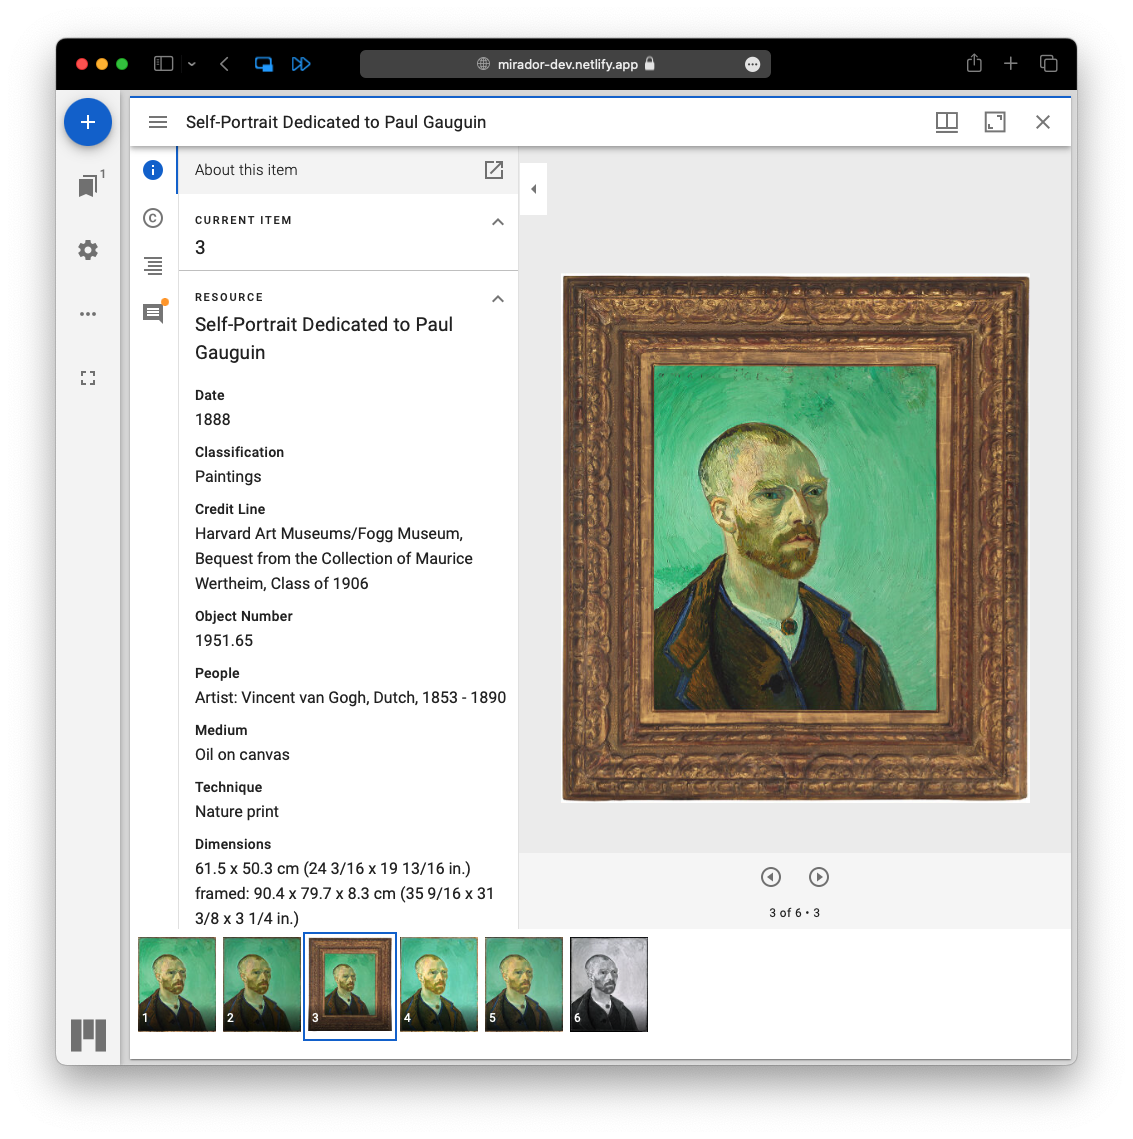
\includegraphics[width=\textwidth]{images/mirador.png}
	\caption{Screenshot of Mirador IIIF Viewer}
	\label{fig:mirador}
\end{figure}